\documentclass[12pt,a4paper]{article}

\usepackage{sbsr}

\title{Metodologia de Análise no Controle de Qualidade \\ de Vetores de Hidrografia e Modelos Digitais de Terreno\\ no Mapeamento do Estado de São Paulo}

\author{Rafael Duarte$^{1}$ \\ Mateus Pedrucci Romanholi$^2$}

\address{$^1$ Instituto Geográfico e Cartográfico -- IGC\\
	Gerência de Cartografia \\
	Rua Boa Vista, 150 - Centro, São Paulo - SP, Brasil \\
	rduarte@sp.br \\ \ \\
			$^2$ Escola Politécnica da Universidade de São Paulo -- Poli/USP\\
			Departamento de Engenharia de Transportes - PTR \\
			Av. Prof. Almeida Prado, Travessa 2, nº 83 - Butantã -- São Paulo - SP, Brasil \\
			mateus.romanholi@usp.br \\ \ \\
}



\paperlanguage{portugues} % change to "english" in case of english paper

\begin{document}
	\maketitle
	\keywords{Methodology of Validation}{quality control}{cartography}
	\palavraschave{Metodologia de Validação}{Controle de Qualidade}{Cartografia}
	\begin{abstract}
This paper describes how cartographic literature has been applied to validate and control the quality, in terms of positional accuracy and topologic consistence, of the vector hidrography and digital terrain models produced in the scope of the mapping project being carried out by the Geographic and Cartographic Institute of the State of São Paulo (Brazil) at 1:25.000 scale. 
	\end{abstract}

	\section{Introdução}
	\label{sec:paginas}
		Segundo \citeonline{leal2002consideraccoes} devido a demanda por produtos cartográficos de
		qualidade satisfatória é necessário estabelecer parâmetros mínimos para o desenvolvimento
		destes produtos. Neste sentido observa-se a necessidade de trabalhos que descrevam processos de controle de qualidade, conforme proposto neste trabalho.
		
		Com a necessidade de normatizar produtos geoespaciais, a International Organization for Standardization - ISO criou a série ISO 19000, que propõem a padronização de dados geoespaciais. A ISO:19157 (\citeyear{ISO19157}), em especial, define formas para classificar a qualidade da informação geoespacial de duas maneiras: posicional e semântica.

		Para a análise semântica dos produtos digitais, foi proposta como norma para aquisição
		de informação geoespacial as Especificações Técnicas para Aquisição de Dados Geoespaciais Vetoriais (ET-ADGV), da Infraestrutura Nacional de Dados Espaciais (INDE), que propõe a padronização da
		aquisição de dados geoespaciais \cite{de2011especificaccao}. A ET-ADGV propõe novos parâmetros em relação
		ao Decreto n$^{\circ}$ 89.817/84, possibilitando o controle de qualidade de produtos digitais.
				
		\section{Revisão Bibliográfica}
		
	    Segundo \citeonline{guptill2013elements} e Fegeas et. al (1992) podemos diferenciar as inconformidades das seguintes formas: qualidade posicional, a linhagem, fidelidade de atributos, completeza, consistência lógica e fidelidade à semântica.
		
	    Segundo \citeonline{miller1958digital}, o Modelo Digital
	    	de Terreno (MDT) ou Digital Terrain Model (DTM), do inglês, é uma representação estatística
	    	da superfície contínua do terreno, por meio de pontos selecionados, com coordenadas X, Y, Z
	    	determinadas, em um dado sistema de coordenadas.
		
		Segundo \citeonline{assessmentblak} as análise de qualidade do MDT são divididos em análises quantitativas e qualitativas. As análises quantitativas são análises que levam em consideração observações das diferenças encontradas entre o modelo e pontos de referência tidos como pontos verdadeiros.As análises qualitativas, por sua vez, levam em consideração comparações que utilizam
		como referência a estatística e a distribuição de amostras pontuais.
		
		Para análises quantitativas de MDT segundo \citeonline{de2011especificaccao} recomenda-se a utilização da ET-ADGV,
		na qual são definidas classes qualitativas de precisão. Este indicador estatístico é o Padrão de
		Exatidão Cartográfica dos Produtos Cartográficos Digitais (PEC-PCD) na figura \ref{fig:Figura1006}. Quanto a avaliação posicional estatística absoluta segundo \citeonline{merchant1982spatial} quando comparados pontos de melhor acurácia com pontos homólogos no produto torna-se possível a aplicação de testes medindo a tendência e precisão do produto. A utilização desta proposta para, visando porem atender ao decreto n$^{\circ}$ 89.817 de 20 de junho de 1984 (\citeauthor{brasil22decreto},1984), foi documentada por \citeonline{galoecamargo}.
		
		\begin{figure}[ht]
			\centering
			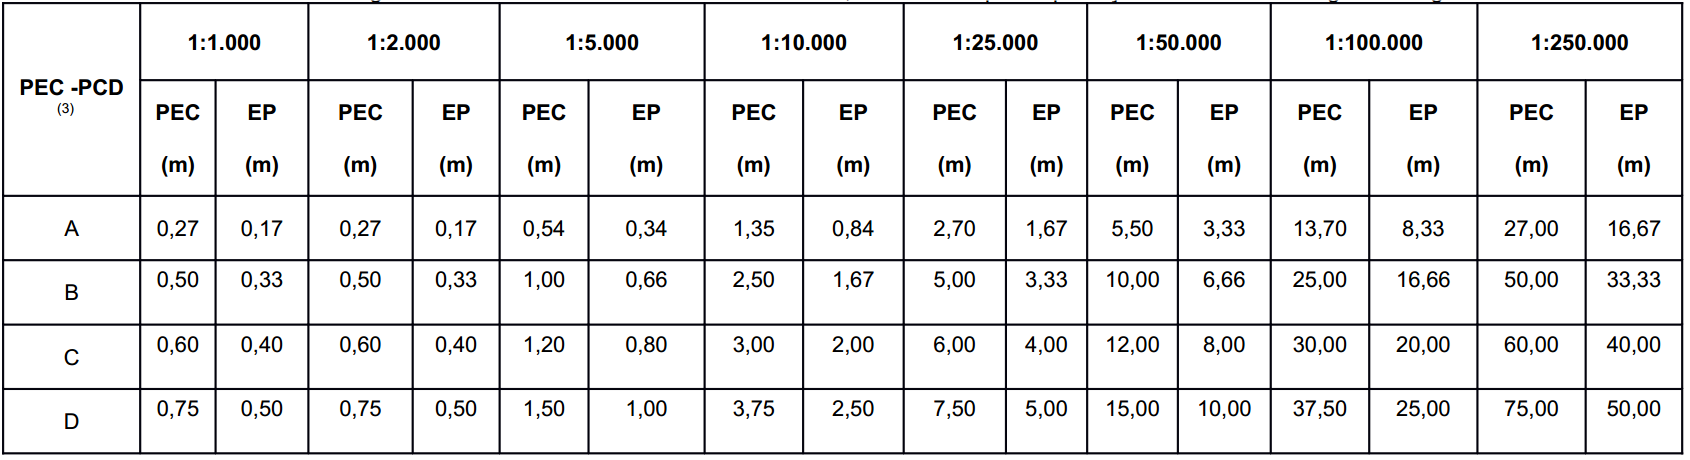
\includegraphics[width=0.7\textwidth]{pecpcd}
			\caption{Valores PEC-PCD para modelos digitais de superfície segundo \cite{de2011especificaccao}}
			\label{fig:Figura1006}
		\end{figure}
		Em análises qualitativas de MDTs \citeonline[p. 443]{assessmentblak} sugere
		utilizar o relevo sombreado (\textit{shaded relief} ou \textit{hillshade}) do MDT, que auxilia na visualização de anomalias no terreno. Quando disponíveis modelos ou
		linhas de quebra (\textit{BreakLine}) podem ser utilizados como boas referências para a verificação.

	    \section{Desenvolvimento}
		Na execução da análise, inicialmente é identificado o produto a ser realizada a análise. Na
		execução deste processo, é necessário efetuar controle e separação conforme demonstrado pelo
		diagrama da figura \ref{diagrama:1}. Após o processo de controle dos arquivos, são executadas as análises dos
		vetores de hidrografia e do MDT.
		% Graphic for TeX using PGF
% Title: E:\projetos_c\sbsr2017\diagrama1.dia
% Creator: Dia v0.97.2
% CreationDate: Wed Oct 12 15:06:25 2016
% For: Katia-PC
% \usepackage{tikz}
% The following commands are not supported in PSTricks at present
% We define them conditionally, so when they are implemented,
% this pgf file will use them.
\begin{figure}
\centering

\ifx\du\undefined
  \newlength{\du}
\fi
\setlength{\du}{15\unitlength}

\begin{tikzpicture}[thick,scale=0.4, every node/.style={scale=0.3}]
\pgftransformxscale{1.000000}
\pgftransformyscale{-1.000000}
\definecolor{dialinecolor}{rgb}{0.000000, 0.000000, 0.000000}
\pgfsetstrokecolor{dialinecolor}
\definecolor{dialinecolor}{rgb}{1.000000, 1.000000, 1.000000}
\pgfsetfillcolor{dialinecolor}
\pgfsetlinewidth{0.100000\du}
\pgfsetdash{}{0pt}
\pgfsetdash{}{0pt}
\pgfsetbuttcap
\pgfsetmiterjoin
\pgfsetlinewidth{0.100000\du}
\pgfsetbuttcap
\pgfsetmiterjoin
\pgfsetdash{}{0pt}
\definecolor{dialinecolor}{rgb}{1.000000, 1.000000, 1.000000}
\pgfsetfillcolor{dialinecolor}
\pgfpathmoveto{\pgfpoint{9.050000\du}{10.083333\du}}
\pgfpathcurveto{\pgfpoint{9.720000\du}{9.608333\du}}{\pgfpoint{10.055000\du}{9.450000\du}}{\pgfpoint{10.725000\du}{9.450000\du}}
\pgfpathcurveto{\pgfpoint{11.395000\du}{9.450000\du}}{\pgfpoint{11.730000\du}{9.608333\du}}{\pgfpoint{12.400000\du}{10.083333\du}}
\pgfpathlineto{\pgfpoint{12.400000\du}{12.616667\du}}
\pgfpathcurveto{\pgfpoint{11.730000\du}{13.091667\du}}{\pgfpoint{11.395000\du}{13.250000\du}}{\pgfpoint{10.725000\du}{13.250000\du}}
\pgfpathcurveto{\pgfpoint{10.055000\du}{13.250000\du}}{\pgfpoint{9.720000\du}{13.091667\du}}{\pgfpoint{9.050000\du}{12.616667\du}}
\pgfpathlineto{\pgfpoint{9.050000\du}{10.083333\du}}
\pgfusepath{fill}
\definecolor{dialinecolor}{rgb}{0.000000, 0.000000, 0.000000}
\pgfsetstrokecolor{dialinecolor}
\pgfpathmoveto{\pgfpoint{9.050000\du}{10.083333\du}}
\pgfpathcurveto{\pgfpoint{9.720000\du}{9.608333\du}}{\pgfpoint{10.055000\du}{9.450000\du}}{\pgfpoint{10.725000\du}{9.450000\du}}
\pgfpathcurveto{\pgfpoint{11.395000\du}{9.450000\du}}{\pgfpoint{11.730000\du}{9.608333\du}}{\pgfpoint{12.400000\du}{10.083333\du}}
\pgfpathlineto{\pgfpoint{12.400000\du}{12.616667\du}}
\pgfpathcurveto{\pgfpoint{11.730000\du}{13.091667\du}}{\pgfpoint{11.395000\du}{13.250000\du}}{\pgfpoint{10.725000\du}{13.250000\du}}
\pgfpathcurveto{\pgfpoint{10.055000\du}{13.250000\du}}{\pgfpoint{9.720000\du}{13.091667\du}}{\pgfpoint{9.050000\du}{12.616667\du}}
\pgfpathlineto{\pgfpoint{9.050000\du}{10.083333\du}}
\pgfusepath{stroke}
\pgfsetbuttcap
\pgfsetmiterjoin
\pgfsetdash{}{0pt}
\definecolor{dialinecolor}{rgb}{0.000000, 0.000000, 0.000000}
\pgfsetstrokecolor{dialinecolor}
\pgfpathmoveto{\pgfpoint{9.050000\du}{10.083333\du}}
\pgfpathcurveto{\pgfpoint{9.720000\du}{10.558333\du}}{\pgfpoint{10.055000\du}{10.716667\du}}{\pgfpoint{10.725000\du}{10.716667\du}}
\pgfpathcurveto{\pgfpoint{11.395000\du}{10.716667\du}}{\pgfpoint{11.730000\du}{10.558333\du}}{\pgfpoint{12.400000\du}{10.083333\du}}
\pgfusepath{stroke}
% setfont left to latex
\definecolor{dialinecolor}{rgb}{0.000000, 0.000000, 0.000000}
\pgfsetstrokecolor{dialinecolor}
\node at (10.725000\du,11.506667\du){Arquivos};
% setfont left to latex
\definecolor{dialinecolor}{rgb}{0.000000, 0.000000, 0.000000}
\pgfsetstrokecolor{dialinecolor}
\node at (10.725000\du,12.306667\du){Recebidos};
\pgfsetlinewidth{0.100000\du}
\pgfsetdash{}{0pt}
\pgfsetdash{}{0pt}
\pgfsetbuttcap
{
\definecolor{dialinecolor}{rgb}{0.000000, 0.000000, 0.000000}
\pgfsetfillcolor{dialinecolor}
% was here!!!
\pgfsetarrowsend{stealth}
\definecolor{dialinecolor}{rgb}{0.000000, 0.000000, 0.000000}
\pgfsetstrokecolor{dialinecolor}
\draw (12.400000\du,11.033333\du)--(17.120662\du,11.025000\du);
}
\definecolor{dialinecolor}{rgb}{1.000000, 1.000000, 1.000000}
\pgfsetfillcolor{dialinecolor}
\fill (17.712114\du,9.400000\du)--(21.470790\du,9.400000\du)--(20.287886\du,12.650000\du)--(16.529210\du,12.650000\du)--cycle;
\pgfsetlinewidth{0.100000\du}
\pgfsetdash{}{0pt}
\pgfsetdash{}{0pt}
\pgfsetmiterjoin
\definecolor{dialinecolor}{rgb}{0.000000, 0.000000, 0.000000}
\pgfsetstrokecolor{dialinecolor}
\draw (17.712114\du,9.400000\du)--(21.470790\du,9.400000\du)--(20.287886\du,12.650000\du)--(16.529210\du,12.650000\du)--cycle;
% setfont left to latex
\definecolor{dialinecolor}{rgb}{0.000000, 0.000000, 0.000000}
\pgfsetstrokecolor{dialinecolor}
\node at (19.000000\du,11.265000\du){Controle};
\pgfsetlinewidth{0.100000\du}
\pgfsetdash{}{0pt}
\pgfsetdash{}{0pt}
\pgfsetbuttcap
\pgfsetmiterjoin
\pgfsetlinewidth{0.100000\du}
\pgfsetbuttcap
\pgfsetmiterjoin
\pgfsetdash{}{0pt}
\definecolor{dialinecolor}{rgb}{1.000000, 1.000000, 1.000000}
\pgfsetfillcolor{dialinecolor}
\pgfpathmoveto{\pgfpoint{25.000000\du}{9.600000\du}}
\pgfpathlineto{\pgfpoint{28.850000\du}{9.600000\du}}
\pgfpathlineto{\pgfpoint{28.850000\du}{12.557143\du}}
\pgfpathcurveto{\pgfpoint{28.080000\du}{12.064286\du}}{\pgfpoint{27.695000\du}{12.064286\du}}{\pgfpoint{26.925000\du}{12.557143\du}}
\pgfpathcurveto{\pgfpoint{26.155000\du}{13.050000\du}}{\pgfpoint{25.770000\du}{13.050000\du}}{\pgfpoint{25.000000\du}{12.557143\du}}
\pgfpathlineto{\pgfpoint{25.000000\du}{9.600000\du}}
\pgfusepath{fill}
\definecolor{dialinecolor}{rgb}{0.000000, 0.000000, 0.000000}
\pgfsetstrokecolor{dialinecolor}
\pgfpathmoveto{\pgfpoint{25.000000\du}{9.600000\du}}
\pgfpathlineto{\pgfpoint{28.850000\du}{9.600000\du}}
\pgfpathlineto{\pgfpoint{28.850000\du}{12.557143\du}}
\pgfpathcurveto{\pgfpoint{28.080000\du}{12.064286\du}}{\pgfpoint{27.695000\du}{12.064286\du}}{\pgfpoint{26.925000\du}{12.557143\du}}
\pgfpathcurveto{\pgfpoint{26.155000\du}{13.050000\du}}{\pgfpoint{25.770000\du}{13.050000\du}}{\pgfpoint{25.000000\du}{12.557143\du}}
\pgfpathlineto{\pgfpoint{25.000000\du}{9.600000\du}}
\pgfusepath{stroke}
% setfont left to latex
\definecolor{dialinecolor}{rgb}{0.000000, 0.000000, 0.000000}
\pgfsetstrokecolor{dialinecolor}
\node at (26.925000\du,10.672143\du){Relatório};
% setfont left to latex
\definecolor{dialinecolor}{rgb}{0.000000, 0.000000, 0.000000}
\pgfsetstrokecolor{dialinecolor}
\node at (26.925000\du,11.472143\du){Geoportal};
\pgfsetlinewidth{0.100000\du}
\pgfsetdash{}{0pt}
\pgfsetdash{}{0pt}
\pgfsetbuttcap
{
\definecolor{dialinecolor}{rgb}{0.000000, 0.000000, 0.000000}
\pgfsetfillcolor{dialinecolor}
% was here!!!
\pgfsetarrowsend{stealth}
\definecolor{dialinecolor}{rgb}{0.000000, 0.000000, 0.000000}
\pgfsetstrokecolor{dialinecolor}
\draw (20.879338\du,11.025000\du)--(25.000000\du,11.078571\du);
}
\pgfsetlinewidth{0.100000\du}
\pgfsetdash{}{0pt}
\pgfsetdash{}{0pt}
\pgfsetbuttcap
\pgfsetmiterjoin
\pgfsetlinewidth{0.100000\du}
\pgfsetbuttcap
\pgfsetmiterjoin
\pgfsetdash{}{0pt}
\definecolor{dialinecolor}{rgb}{1.000000, 1.000000, 1.000000}
\pgfsetfillcolor{dialinecolor}
\pgfpathmoveto{\pgfpoint{7.890000\du}{19.100000\du}}
\pgfpathlineto{\pgfpoint{11.310000\du}{19.100000\du}}
\pgfpathlineto{\pgfpoint{11.994000\du}{20.450000\du}}
\pgfpathlineto{\pgfpoint{11.310000\du}{21.800000\du}}
\pgfpathlineto{\pgfpoint{7.890000\du}{21.800000\du}}
\pgfpathlineto{\pgfpoint{7.206000\du}{20.450000\du}}
\pgfpathlineto{\pgfpoint{7.890000\du}{19.100000\du}}
\pgfusepath{fill}
\definecolor{dialinecolor}{rgb}{0.000000, 0.000000, 0.000000}
\pgfsetstrokecolor{dialinecolor}
\pgfpathmoveto{\pgfpoint{7.890000\du}{19.100000\du}}
\pgfpathlineto{\pgfpoint{11.310000\du}{19.100000\du}}
\pgfpathlineto{\pgfpoint{11.994000\du}{20.450000\du}}
\pgfpathlineto{\pgfpoint{11.310000\du}{21.800000\du}}
\pgfpathlineto{\pgfpoint{7.890000\du}{21.800000\du}}
\pgfpathlineto{\pgfpoint{7.206000\du}{20.450000\du}}
\pgfpathlineto{\pgfpoint{7.890000\du}{19.100000\du}}
\pgfusepath{stroke}
% setfont left to latex
\definecolor{dialinecolor}{rgb}{0.000000, 0.000000, 0.000000}
\pgfsetstrokecolor{dialinecolor}
\node at (9.600000\du,20.290000\du){Vetor};
% setfont left to latex
\definecolor{dialinecolor}{rgb}{0.000000, 0.000000, 0.000000}
\pgfsetstrokecolor{dialinecolor}
\node at (9.600000\du,21.090000\du){Hidrografia};
\definecolor{dialinecolor}{rgb}{1.000000, 1.000000, 1.000000}
\pgfsetfillcolor{dialinecolor}
\fill (18.444630\du,14.244700\du)--(19.749960\du,15.572365\du)--(18.444630\du,16.900030\du)--(17.139300\du,15.572365\du)--cycle;
\pgfsetlinewidth{0.100000\du}
\pgfsetdash{}{0pt}
\pgfsetdash{}{0pt}
\pgfsetmiterjoin
\definecolor{dialinecolor}{rgb}{0.000000, 0.000000, 0.000000}
\pgfsetstrokecolor{dialinecolor}
\draw (18.444630\du,14.244700\du)--(19.749960\du,15.572365\du)--(18.444630\du,16.900030\du)--(17.139300\du,15.572365\du)--cycle;
% setfont left to latex
\definecolor{dialinecolor}{rgb}{0.000000, 0.000000, 0.000000}
\pgfsetstrokecolor{dialinecolor}
\node at (18.444630\du,15.812365\du){};
\pgfsetlinewidth{0.100000\du}
\pgfsetdash{}{0pt}
\pgfsetdash{}{0pt}
\pgfsetbuttcap
\pgfsetmiterjoin
\pgfsetlinewidth{0.100000\du}
\pgfsetbuttcap
\pgfsetmiterjoin
\pgfsetdash{}{0pt}
\definecolor{dialinecolor}{rgb}{1.000000, 1.000000, 1.000000}
\pgfsetfillcolor{dialinecolor}
\pgfpathmoveto{\pgfpoint{25.190000\du}{19.100000\du}}
\pgfpathlineto{\pgfpoint{29.260000\du}{19.100000\du}}
\pgfpathlineto{\pgfpoint{30.074000\du}{20.450000\du}}
\pgfpathlineto{\pgfpoint{29.260000\du}{21.800000\du}}
\pgfpathlineto{\pgfpoint{25.190000\du}{21.800000\du}}
\pgfpathlineto{\pgfpoint{24.376000\du}{20.450000\du}}
\pgfpathlineto{\pgfpoint{25.190000\du}{19.100000\du}}
\pgfusepath{fill}
\definecolor{dialinecolor}{rgb}{0.000000, 0.000000, 0.000000}
\pgfsetstrokecolor{dialinecolor}
\pgfpathmoveto{\pgfpoint{25.190000\du}{19.100000\du}}
\pgfpathlineto{\pgfpoint{29.260000\du}{19.100000\du}}
\pgfpathlineto{\pgfpoint{30.074000\du}{20.450000\du}}
\pgfpathlineto{\pgfpoint{29.260000\du}{21.800000\du}}
\pgfpathlineto{\pgfpoint{25.190000\du}{21.800000\du}}
\pgfpathlineto{\pgfpoint{24.376000\du}{20.450000\du}}
\pgfpathlineto{\pgfpoint{25.190000\du}{19.100000\du}}
\pgfusepath{stroke}
% setfont left to latex
\definecolor{dialinecolor}{rgb}{0.000000, 0.000000, 0.000000}
\pgfsetstrokecolor{dialinecolor}
\node at (27.225000\du,20.290000\du){Ortomosaico};
% setfont left to latex
\definecolor{dialinecolor}{rgb}{0.000000, 0.000000, 0.000000}
\pgfsetstrokecolor{dialinecolor}
\node at (27.225000\du,21.090000\du){Ortofotocarta};
\pgfsetlinewidth{0.100000\du}
\pgfsetdash{}{0pt}
\pgfsetdash{}{0pt}
\pgfsetbuttcap
{
\definecolor{dialinecolor}{rgb}{0.000000, 0.000000, 0.000000}
\pgfsetfillcolor{dialinecolor}
% was here!!!
\pgfsetarrowsend{stealth}
\definecolor{dialinecolor}{rgb}{0.000000, 0.000000, 0.000000}
\pgfsetstrokecolor{dialinecolor}
\draw (18.408548\du,12.650000\du)--(18.444700\du,14.244700\du);
}
\pgfsetlinewidth{0.100000\du}
\pgfsetdash{}{0pt}
\pgfsetdash{}{0pt}
\pgfsetmiterjoin
\pgfsetbuttcap
{
\definecolor{dialinecolor}{rgb}{0.000000, 0.000000, 0.000000}
\pgfsetfillcolor{dialinecolor}
% was here!!!
\pgfsetarrowsend{stealth}
{\pgfsetcornersarced{\pgfpoint{0.000000\du}{0.000000\du}}\definecolor{dialinecolor}{rgb}{0.000000, 0.000000, 0.000000}
\pgfsetstrokecolor{dialinecolor}
\draw (19.750000\du,15.572300\du)--(22.250000\du,15.572300\du)--(22.250000\du,20.450000\du)--(24.376000\du,20.450000\du);
}}
\pgfsetlinewidth{0.100000\du}
\pgfsetdash{}{0pt}
\pgfsetdash{}{0pt}
\pgfsetmiterjoin
\pgfsetbuttcap
{
\definecolor{dialinecolor}{rgb}{0.000000, 0.000000, 0.000000}
\pgfsetfillcolor{dialinecolor}
% was here!!!
\pgfsetarrowsend{stealth}
{\pgfsetcornersarced{\pgfpoint{0.000000\du}{0.000000\du}}\definecolor{dialinecolor}{rgb}{0.000000, 0.000000, 0.000000}
\pgfsetstrokecolor{dialinecolor}
\draw (17.139300\du,15.572300\du)--(17.139300\du,15.600000\du)--(14.250000\du,15.600000\du)--(14.250000\du,20.450000\du)--(11.994000\du,20.450000\du);
}}
\pgfsetlinewidth{0.100000\du}
\pgfsetdash{}{0pt}
\pgfsetdash{}{0pt}
\pgfsetbuttcap
\pgfsetmiterjoin
\pgfsetlinewidth{0.100000\du}
\pgfsetbuttcap
\pgfsetmiterjoin
\pgfsetdash{}{0pt}
\definecolor{dialinecolor}{rgb}{1.000000, 1.000000, 1.000000}
\pgfsetfillcolor{dialinecolor}
\fill (7.350000\du,25.550000\du)--(7.350000\du,29.100000\du)--(11.850000\du,29.100000\du)--(11.850000\du,25.550000\du)--cycle;
\definecolor{dialinecolor}{rgb}{0.000000, 0.000000, 0.000000}
\pgfsetstrokecolor{dialinecolor}
\draw (7.350000\du,25.550000\du)--(7.350000\du,29.100000\du)--(11.850000\du,29.100000\du)--(11.850000\du,25.550000\du)--cycle;
\pgfsetbuttcap
\pgfsetmiterjoin
\pgfsetdash{}{0pt}
\definecolor{dialinecolor}{rgb}{0.000000, 0.000000, 0.000000}
\pgfsetstrokecolor{dialinecolor}
\draw (7.800000\du,25.550000\du)--(7.800000\du,29.100000\du);
\pgfsetbuttcap
\pgfsetmiterjoin
\pgfsetdash{}{0pt}
\definecolor{dialinecolor}{rgb}{0.000000, 0.000000, 0.000000}
\pgfsetstrokecolor{dialinecolor}
\draw (11.400000\du,25.550000\du)--(11.400000\du,29.100000\du);
% setfont left to latex
\definecolor{dialinecolor}{rgb}{0.000000, 0.000000, 0.000000}
\pgfsetstrokecolor{dialinecolor}
\node at (9.600000\du,26.765000\du){Análise};
% setfont left to latex
\definecolor{dialinecolor}{rgb}{0.000000, 0.000000, 0.000000}
\pgfsetstrokecolor{dialinecolor}
\node at (9.600000\du,27.565000\du){Hidrografia};
% setfont left to latex
\definecolor{dialinecolor}{rgb}{0.000000, 0.000000, 0.000000}
\pgfsetstrokecolor{dialinecolor}
\node at (9.600000\du,28.365000\du){Editada};
\pgfsetlinewidth{0.100000\du}
\pgfsetdash{}{0pt}
\pgfsetdash{}{0pt}
\pgfsetbuttcap
\pgfsetmiterjoin
\pgfsetlinewidth{0.100000\du}
\pgfsetbuttcap
\pgfsetmiterjoin
\pgfsetdash{}{0pt}
\definecolor{dialinecolor}{rgb}{1.000000, 1.000000, 1.000000}
\pgfsetfillcolor{dialinecolor}
\pgfpathmoveto{\pgfpoint{16.747300\du}{18.950000\du}}
\pgfpathlineto{\pgfpoint{20.167300\du}{18.950000\du}}
\pgfpathlineto{\pgfpoint{20.851300\du}{20.450000\du}}
\pgfpathlineto{\pgfpoint{20.167300\du}{21.950000\du}}
\pgfpathlineto{\pgfpoint{16.747300\du}{21.950000\du}}
\pgfpathlineto{\pgfpoint{16.063300\du}{20.450000\du}}
\pgfpathlineto{\pgfpoint{16.747300\du}{18.950000\du}}
\pgfusepath{fill}
\definecolor{dialinecolor}{rgb}{0.000000, 0.000000, 0.000000}
\pgfsetstrokecolor{dialinecolor}
\pgfpathmoveto{\pgfpoint{16.747300\du}{18.950000\du}}
\pgfpathlineto{\pgfpoint{20.167300\du}{18.950000\du}}
\pgfpathlineto{\pgfpoint{20.851300\du}{20.450000\du}}
\pgfpathlineto{\pgfpoint{20.167300\du}{21.950000\du}}
\pgfpathlineto{\pgfpoint{16.747300\du}{21.950000\du}}
\pgfpathlineto{\pgfpoint{16.063300\du}{20.450000\du}}
\pgfpathlineto{\pgfpoint{16.747300\du}{18.950000\du}}
\pgfusepath{stroke}
% setfont left to latex
\definecolor{dialinecolor}{rgb}{0.000000, 0.000000, 0.000000}
\pgfsetstrokecolor{dialinecolor}
\node at (18.457300\du,19.890000\du){Modelo};
% setfont left to latex
\definecolor{dialinecolor}{rgb}{0.000000, 0.000000, 0.000000}
\pgfsetstrokecolor{dialinecolor}
\node at (18.457300\du,20.690000\du){Digital};
% setfont left to latex
\definecolor{dialinecolor}{rgb}{0.000000, 0.000000, 0.000000}
\pgfsetstrokecolor{dialinecolor}
\node at (18.457300\du,21.490000\du){Terreno};
\pgfsetlinewidth{0.100000\du}
\pgfsetdash{}{0pt}
\pgfsetdash{}{0pt}
\pgfsetbuttcap
{
\definecolor{dialinecolor}{rgb}{0.000000, 0.000000, 0.000000}
\pgfsetfillcolor{dialinecolor}
% was here!!!
\pgfsetarrowsend{stealth}
\definecolor{dialinecolor}{rgb}{0.000000, 0.000000, 0.000000}
\pgfsetstrokecolor{dialinecolor}
\draw (18.444700\du,16.900000\du)--(18.457300\du,18.950000\du);
}
\pgfsetlinewidth{0.100000\du}
\pgfsetdash{}{0pt}
\pgfsetdash{}{0pt}
\pgfsetbuttcap
\pgfsetmiterjoin
\pgfsetlinewidth{0.100000\du}
\pgfsetbuttcap
\pgfsetmiterjoin
\pgfsetdash{}{0pt}
\definecolor{dialinecolor}{rgb}{1.000000, 1.000000, 1.000000}
\pgfsetfillcolor{dialinecolor}
\fill (24.781200\du,25.595000\du)--(24.781200\du,29.145000\du)--(29.868700\du,29.145000\du)--(29.868700\du,25.595000\du)--cycle;
\definecolor{dialinecolor}{rgb}{0.000000, 0.000000, 0.000000}
\pgfsetstrokecolor{dialinecolor}
\draw (24.781200\du,25.595000\du)--(24.781200\du,29.145000\du)--(29.868700\du,29.145000\du)--(29.868700\du,25.595000\du)--cycle;
\pgfsetbuttcap
\pgfsetmiterjoin
\pgfsetdash{}{0pt}
\definecolor{dialinecolor}{rgb}{0.000000, 0.000000, 0.000000}
\pgfsetstrokecolor{dialinecolor}
\draw (25.289950\du,25.595000\du)--(25.289950\du,29.145000\du);
\pgfsetbuttcap
\pgfsetmiterjoin
\pgfsetdash{}{0pt}
\definecolor{dialinecolor}{rgb}{0.000000, 0.000000, 0.000000}
\pgfsetstrokecolor{dialinecolor}
\draw (29.359950\du,25.595000\du)--(29.359950\du,29.145000\du);
% setfont left to latex
\definecolor{dialinecolor}{rgb}{0.000000, 0.000000, 0.000000}
\pgfsetstrokecolor{dialinecolor}
\node at (27.324950\du,26.810000\du){Análise};
% setfont left to latex
\definecolor{dialinecolor}{rgb}{0.000000, 0.000000, 0.000000}
\pgfsetstrokecolor{dialinecolor}
\node at (27.324950\du,27.610000\du){Ortofotocarta};
% setfont left to latex
\definecolor{dialinecolor}{rgb}{0.000000, 0.000000, 0.000000}
\pgfsetstrokecolor{dialinecolor}
\node at (27.324950\du,28.410000\du){Editorada};
\pgfsetlinewidth{0.100000\du}
\pgfsetdash{}{0pt}
\pgfsetdash{}{0pt}
\pgfsetbuttcap
\pgfsetmiterjoin
\pgfsetlinewidth{0.100000\du}
\pgfsetbuttcap
\pgfsetmiterjoin
\pgfsetdash{}{0pt}
\definecolor{dialinecolor}{rgb}{1.000000, 1.000000, 1.000000}
\pgfsetfillcolor{dialinecolor}
\fill (16.165600\du,25.540000\du)--(16.165600\du,29.090000\du)--(20.665600\du,29.090000\du)--(20.665600\du,25.540000\du)--cycle;
\definecolor{dialinecolor}{rgb}{0.000000, 0.000000, 0.000000}
\pgfsetstrokecolor{dialinecolor}
\draw (16.165600\du,25.540000\du)--(16.165600\du,29.090000\du)--(20.665600\du,29.090000\du)--(20.665600\du,25.540000\du)--cycle;
\pgfsetbuttcap
\pgfsetmiterjoin
\pgfsetdash{}{0pt}
\definecolor{dialinecolor}{rgb}{0.000000, 0.000000, 0.000000}
\pgfsetstrokecolor{dialinecolor}
\draw (16.615600\du,25.540000\du)--(16.615600\du,29.090000\du);
\pgfsetbuttcap
\pgfsetmiterjoin
\pgfsetdash{}{0pt}
\definecolor{dialinecolor}{rgb}{0.000000, 0.000000, 0.000000}
\pgfsetstrokecolor{dialinecolor}
\draw (20.215600\du,25.540000\du)--(20.215600\du,29.090000\du);
% setfont left to latex
\definecolor{dialinecolor}{rgb}{0.000000, 0.000000, 0.000000}
\pgfsetstrokecolor{dialinecolor}
\node at (18.415600\du,26.755000\du){Análise};
% setfont left to latex
\definecolor{dialinecolor}{rgb}{0.000000, 0.000000, 0.000000}
\pgfsetstrokecolor{dialinecolor}
\node at (18.415600\du,27.555000\du){M.D.T.};
% setfont left to latex
\definecolor{dialinecolor}{rgb}{0.000000, 0.000000, 0.000000}
\pgfsetstrokecolor{dialinecolor}
\node at (18.415600\du,28.355000\du){Editado};
\pgfsetlinewidth{0.100000\du}
\pgfsetdash{}{0pt}
\pgfsetdash{}{0pt}
\pgfsetbuttcap
{
\definecolor{dialinecolor}{rgb}{0.000000, 0.000000, 0.000000}
\pgfsetfillcolor{dialinecolor}
% was here!!!
\pgfsetarrowsend{stealth}
\definecolor{dialinecolor}{rgb}{0.000000, 0.000000, 0.000000}
\pgfsetstrokecolor{dialinecolor}
\draw (9.600000\du,21.800000\du)--(9.600000\du,25.550000\du);
}
\pgfsetlinewidth{0.100000\du}
\pgfsetdash{}{0pt}
\pgfsetdash{}{0pt}
\pgfsetbuttcap
{
\definecolor{dialinecolor}{rgb}{0.000000, 0.000000, 0.000000}
\pgfsetfillcolor{dialinecolor}
% was here!!!
\pgfsetarrowsend{stealth}
\definecolor{dialinecolor}{rgb}{0.000000, 0.000000, 0.000000}
\pgfsetstrokecolor{dialinecolor}
\draw (18.457300\du,21.950000\du)--(18.415600\du,25.540000\du);
}
\pgfsetlinewidth{0.100000\du}
\pgfsetdash{}{0pt}
\pgfsetdash{}{0pt}
\pgfsetbuttcap
{
\definecolor{dialinecolor}{rgb}{0.000000, 0.000000, 0.000000}
\pgfsetfillcolor{dialinecolor}
% was here!!!
\pgfsetarrowsend{stealth}
\definecolor{dialinecolor}{rgb}{0.000000, 0.000000, 0.000000}
\pgfsetstrokecolor{dialinecolor}
\draw (27.225000\du,21.800000\du)--(27.324950\du,25.595000\du);
}
% setfont left to latex
\definecolor{dialinecolor}{rgb}{0.000000, 0.000000, 0.000000}
\pgfsetstrokecolor{dialinecolor}
\node[anchor=west] at (19.700000\du,14.250000\du){Separação};
\pgfsetlinewidth{0.100000\du}
\pgfsetdash{}{0pt}
\pgfsetdash{}{0pt}
\pgfsetbuttcap
\pgfsetmiterjoin
\pgfsetlinewidth{0.100000\du}
\pgfsetbuttcap
\pgfsetmiterjoin
\pgfsetdash{}{0pt}
\definecolor{dialinecolor}{rgb}{1.000000, 1.000000, 1.000000}
\pgfsetfillcolor{dialinecolor}
\pgfpathmoveto{\pgfpoint{7.450000\du}{31.747500\du}}
\pgfpathcurveto{\pgfpoint{8.300000\du}{31.250625\du}}{\pgfpoint{8.725000\du}{31.085000\du}}{\pgfpoint{9.575000\du}{31.085000\du}}
\pgfpathcurveto{\pgfpoint{10.425000\du}{31.085000\du}}{\pgfpoint{10.850000\du}{31.250625\du}}{\pgfpoint{11.700000\du}{31.747500\du}}
\pgfpathlineto{\pgfpoint{11.700000\du}{34.397500\du}}
\pgfpathcurveto{\pgfpoint{10.850000\du}{34.894375\du}}{\pgfpoint{10.425000\du}{35.060000\du}}{\pgfpoint{9.575000\du}{35.060000\du}}
\pgfpathcurveto{\pgfpoint{8.725000\du}{35.060000\du}}{\pgfpoint{8.300000\du}{34.894375\du}}{\pgfpoint{7.450000\du}{34.397500\du}}
\pgfpathlineto{\pgfpoint{7.450000\du}{31.747500\du}}
\pgfusepath{fill}
\definecolor{dialinecolor}{rgb}{0.000000, 0.000000, 0.000000}
\pgfsetstrokecolor{dialinecolor}
\pgfpathmoveto{\pgfpoint{7.450000\du}{31.747500\du}}
\pgfpathcurveto{\pgfpoint{8.300000\du}{31.250625\du}}{\pgfpoint{8.725000\du}{31.085000\du}}{\pgfpoint{9.575000\du}{31.085000\du}}
\pgfpathcurveto{\pgfpoint{10.425000\du}{31.085000\du}}{\pgfpoint{10.850000\du}{31.250625\du}}{\pgfpoint{11.700000\du}{31.747500\du}}
\pgfpathlineto{\pgfpoint{11.700000\du}{34.397500\du}}
\pgfpathcurveto{\pgfpoint{10.850000\du}{34.894375\du}}{\pgfpoint{10.425000\du}{35.060000\du}}{\pgfpoint{9.575000\du}{35.060000\du}}
\pgfpathcurveto{\pgfpoint{8.725000\du}{35.060000\du}}{\pgfpoint{8.300000\du}{34.894375\du}}{\pgfpoint{7.450000\du}{34.397500\du}}
\pgfpathlineto{\pgfpoint{7.450000\du}{31.747500\du}}
\pgfusepath{stroke}
\pgfsetbuttcap
\pgfsetmiterjoin
\pgfsetdash{}{0pt}
\definecolor{dialinecolor}{rgb}{0.000000, 0.000000, 0.000000}
\pgfsetstrokecolor{dialinecolor}
\pgfpathmoveto{\pgfpoint{7.450000\du}{31.747500\du}}
\pgfpathcurveto{\pgfpoint{8.300000\du}{32.244375\du}}{\pgfpoint{8.725000\du}{32.410000\du}}{\pgfpoint{9.575000\du}{32.410000\du}}
\pgfpathcurveto{\pgfpoint{10.425000\du}{32.410000\du}}{\pgfpoint{10.850000\du}{32.244375\du}}{\pgfpoint{11.700000\du}{31.747500\du}}
\pgfusepath{stroke}
% setfont left to latex
\definecolor{dialinecolor}{rgb}{0.000000, 0.000000, 0.000000}
\pgfsetstrokecolor{dialinecolor}
\node at (9.575000\du,33.243750\du){Vetor};
% setfont left to latex
\definecolor{dialinecolor}{rgb}{0.000000, 0.000000, 0.000000}
\pgfsetstrokecolor{dialinecolor}
\node at (9.575000\du,34.043750\du){Aprovado};
\pgfsetlinewidth{0.100000\du}
\pgfsetdash{}{0pt}
\pgfsetdash{}{0pt}
\pgfsetbuttcap
{
\definecolor{dialinecolor}{rgb}{0.000000, 0.000000, 0.000000}
\pgfsetfillcolor{dialinecolor}
% was here!!!
\pgfsetarrowsend{stealth}
\definecolor{dialinecolor}{rgb}{0.000000, 0.000000, 0.000000}
\pgfsetstrokecolor{dialinecolor}
\draw (9.600000\du,29.100000\du)--(9.575000\du,31.085000\du);
}
\pgfsetlinewidth{0.100000\du}
\pgfsetdash{}{0pt}
\pgfsetdash{}{0pt}
\pgfsetbuttcap
\pgfsetmiterjoin
\pgfsetlinewidth{0.100000\du}
\pgfsetbuttcap
\pgfsetmiterjoin
\pgfsetdash{}{0pt}
\definecolor{dialinecolor}{rgb}{1.000000, 1.000000, 1.000000}
\pgfsetfillcolor{dialinecolor}
\pgfpathmoveto{\pgfpoint{16.282500\du}{31.768333\du}}
\pgfpathcurveto{\pgfpoint{17.142500\du}{31.293333\du}}{\pgfpoint{17.572500\du}{31.135000\du}}{\pgfpoint{18.432500\du}{31.135000\du}}
\pgfpathcurveto{\pgfpoint{19.292500\du}{31.135000\du}}{\pgfpoint{19.722500\du}{31.293333\du}}{\pgfpoint{20.582500\du}{31.768333\du}}
\pgfpathlineto{\pgfpoint{20.582500\du}{34.301667\du}}
\pgfpathcurveto{\pgfpoint{19.722500\du}{34.776667\du}}{\pgfpoint{19.292500\du}{34.935000\du}}{\pgfpoint{18.432500\du}{34.935000\du}}
\pgfpathcurveto{\pgfpoint{17.572500\du}{34.935000\du}}{\pgfpoint{17.142500\du}{34.776667\du}}{\pgfpoint{16.282500\du}{34.301667\du}}
\pgfpathlineto{\pgfpoint{16.282500\du}{31.768333\du}}
\pgfusepath{fill}
\definecolor{dialinecolor}{rgb}{0.000000, 0.000000, 0.000000}
\pgfsetstrokecolor{dialinecolor}
\pgfpathmoveto{\pgfpoint{16.282500\du}{31.768333\du}}
\pgfpathcurveto{\pgfpoint{17.142500\du}{31.293333\du}}{\pgfpoint{17.572500\du}{31.135000\du}}{\pgfpoint{18.432500\du}{31.135000\du}}
\pgfpathcurveto{\pgfpoint{19.292500\du}{31.135000\du}}{\pgfpoint{19.722500\du}{31.293333\du}}{\pgfpoint{20.582500\du}{31.768333\du}}
\pgfpathlineto{\pgfpoint{20.582500\du}{34.301667\du}}
\pgfpathcurveto{\pgfpoint{19.722500\du}{34.776667\du}}{\pgfpoint{19.292500\du}{34.935000\du}}{\pgfpoint{18.432500\du}{34.935000\du}}
\pgfpathcurveto{\pgfpoint{17.572500\du}{34.935000\du}}{\pgfpoint{17.142500\du}{34.776667\du}}{\pgfpoint{16.282500\du}{34.301667\du}}
\pgfpathlineto{\pgfpoint{16.282500\du}{31.768333\du}}
\pgfusepath{stroke}
\pgfsetbuttcap
\pgfsetmiterjoin
\pgfsetdash{}{0pt}
\definecolor{dialinecolor}{rgb}{0.000000, 0.000000, 0.000000}
\pgfsetstrokecolor{dialinecolor}
\pgfpathmoveto{\pgfpoint{16.282500\du}{31.768333\du}}
\pgfpathcurveto{\pgfpoint{17.142500\du}{32.243333\du}}{\pgfpoint{17.572500\du}{32.401667\du}}{\pgfpoint{18.432500\du}{32.401667\du}}
\pgfpathcurveto{\pgfpoint{19.292500\du}{32.401667\du}}{\pgfpoint{19.722500\du}{32.243333\du}}{\pgfpoint{20.582500\du}{31.768333\du}}
\pgfusepath{stroke}
% setfont left to latex
\definecolor{dialinecolor}{rgb}{0.000000, 0.000000, 0.000000}
\pgfsetstrokecolor{dialinecolor}
\node at (18.432500\du,33.191667\du){M.D.T.};
% setfont left to latex
\definecolor{dialinecolor}{rgb}{0.000000, 0.000000, 0.000000}
\pgfsetstrokecolor{dialinecolor}
\node at (18.432500\du,33.991667\du){Aprovado};
% setfont left to latex
\definecolor{dialinecolor}{rgb}{0.000000, 0.000000, 0.000000}
\pgfsetstrokecolor{dialinecolor}
\node[anchor=west] at (18.432500\du,33.035000\du){};
\pgfsetlinewidth{0.100000\du}
\pgfsetdash{}{0pt}
\pgfsetdash{}{0pt}
\pgfsetbuttcap
{
\definecolor{dialinecolor}{rgb}{0.000000, 0.000000, 0.000000}
\pgfsetfillcolor{dialinecolor}
% was here!!!
\pgfsetarrowsend{stealth}
\definecolor{dialinecolor}{rgb}{0.000000, 0.000000, 0.000000}
\pgfsetstrokecolor{dialinecolor}
\draw (11.700000\du,32.741250\du)--(16.282500\du,32.718333\du);
}
\pgfsetlinewidth{0.100000\du}
\pgfsetdash{}{0pt}
\pgfsetdash{}{0pt}
\pgfsetbuttcap
\pgfsetmiterjoin
\pgfsetlinewidth{0.100000\du}
\pgfsetbuttcap
\pgfsetmiterjoin
\pgfsetdash{}{0pt}
\definecolor{dialinecolor}{rgb}{1.000000, 1.000000, 1.000000}
\pgfsetfillcolor{dialinecolor}
\pgfpathmoveto{\pgfpoint{25.165000\du}{31.839167\du}}
\pgfpathcurveto{\pgfpoint{26.042000\du}{31.363542\du}}{\pgfpoint{26.480500\du}{31.205000\du}}{\pgfpoint{27.357500\du}{31.205000\du}}
\pgfpathcurveto{\pgfpoint{28.234500\du}{31.205000\du}}{\pgfpoint{28.673000\du}{31.363542\du}}{\pgfpoint{29.550000\du}{31.839167\du}}
\pgfpathlineto{\pgfpoint{29.550000\du}{34.375833\du}}
\pgfpathcurveto{\pgfpoint{28.673000\du}{34.851458\du}}{\pgfpoint{28.234500\du}{35.010000\du}}{\pgfpoint{27.357500\du}{35.010000\du}}
\pgfpathcurveto{\pgfpoint{26.480500\du}{35.010000\du}}{\pgfpoint{26.042000\du}{34.851458\du}}{\pgfpoint{25.165000\du}{34.375833\du}}
\pgfpathlineto{\pgfpoint{25.165000\du}{31.839167\du}}
\pgfusepath{fill}
\definecolor{dialinecolor}{rgb}{0.000000, 0.000000, 0.000000}
\pgfsetstrokecolor{dialinecolor}
\pgfpathmoveto{\pgfpoint{25.165000\du}{31.839167\du}}
\pgfpathcurveto{\pgfpoint{26.042000\du}{31.363542\du}}{\pgfpoint{26.480500\du}{31.205000\du}}{\pgfpoint{27.357500\du}{31.205000\du}}
\pgfpathcurveto{\pgfpoint{28.234500\du}{31.205000\du}}{\pgfpoint{28.673000\du}{31.363542\du}}{\pgfpoint{29.550000\du}{31.839167\du}}
\pgfpathlineto{\pgfpoint{29.550000\du}{34.375833\du}}
\pgfpathcurveto{\pgfpoint{28.673000\du}{34.851458\du}}{\pgfpoint{28.234500\du}{35.010000\du}}{\pgfpoint{27.357500\du}{35.010000\du}}
\pgfpathcurveto{\pgfpoint{26.480500\du}{35.010000\du}}{\pgfpoint{26.042000\du}{34.851458\du}}{\pgfpoint{25.165000\du}{34.375833\du}}
\pgfpathlineto{\pgfpoint{25.165000\du}{31.839167\du}}
\pgfusepath{stroke}
\pgfsetbuttcap
\pgfsetmiterjoin
\pgfsetdash{}{0pt}
\definecolor{dialinecolor}{rgb}{0.000000, 0.000000, 0.000000}
\pgfsetstrokecolor{dialinecolor}
\pgfpathmoveto{\pgfpoint{25.165000\du}{31.839167\du}}
\pgfpathcurveto{\pgfpoint{26.042000\du}{32.314792\du}}{\pgfpoint{26.480500\du}{32.473333\du}}{\pgfpoint{27.357500\du}{32.473333\du}}
\pgfpathcurveto{\pgfpoint{28.234500\du}{32.473333\du}}{\pgfpoint{28.673000\du}{32.314792\du}}{\pgfpoint{29.550000\du}{31.839167\du}}
\pgfusepath{stroke}
% setfont left to latex
\definecolor{dialinecolor}{rgb}{0.000000, 0.000000, 0.000000}
\pgfsetstrokecolor{dialinecolor}
\node at (27.357500\du,33.264583\du){Ortofotocarta};
% setfont left to latex
\definecolor{dialinecolor}{rgb}{0.000000, 0.000000, 0.000000}
\pgfsetstrokecolor{dialinecolor}
\node at (27.357500\du,34.064583\du){Aprovada};
\pgfsetlinewidth{0.100000\du}
\pgfsetdash{}{0pt}
\pgfsetdash{}{0pt}
\pgfsetbuttcap
{
\definecolor{dialinecolor}{rgb}{0.000000, 0.000000, 0.000000}
\pgfsetfillcolor{dialinecolor}
% was here!!!
\pgfsetarrowsend{stealth}
\definecolor{dialinecolor}{rgb}{0.000000, 0.000000, 0.000000}
\pgfsetstrokecolor{dialinecolor}
\draw (20.582500\du,32.718333\du)--(25.165000\du,32.790417\du);
}
\pgfsetlinewidth{0.100000\du}
\pgfsetdash{}{0pt}
\pgfsetdash{}{0pt}
\pgfsetbuttcap
{
\definecolor{dialinecolor}{rgb}{0.000000, 0.000000, 0.000000}
\pgfsetfillcolor{dialinecolor}
% was here!!!
\pgfsetarrowsend{stealth}
\definecolor{dialinecolor}{rgb}{0.000000, 0.000000, 0.000000}
\pgfsetstrokecolor{dialinecolor}
\draw (18.415600\du,29.090000\du)--(18.432500\du,31.135000\du);
}
\pgfsetlinewidth{0.100000\du}
\pgfsetdash{}{0pt}
\pgfsetdash{}{0pt}
\pgfsetbuttcap
{
\definecolor{dialinecolor}{rgb}{0.000000, 0.000000, 0.000000}
\pgfsetfillcolor{dialinecolor}
% was here!!!
\pgfsetarrowsend{stealth}
\definecolor{dialinecolor}{rgb}{0.000000, 0.000000, 0.000000}
\pgfsetstrokecolor{dialinecolor}
\draw (27.324950\du,29.145000\du)--(27.357500\du,31.205000\du);
}

\end{tikzpicture}
\caption{Diagrama de separação e organização para análise} \label{diagrama:1}
\end{figure}
		Após o processo de controle dos arquivos serão descritas as analises do vetor de hidrografia editada e do MDT.
		\subsection{Descrição das análises efetuadas nos Vetores de Hidrografia}
		A seguir serão detalhadas as análises efetuadas na rede hidrográfica vetorial que foram agrupadas em: Consistência Lógica (fidelidade de atributos, fidelidade à semântica), Completititude e Acurácia Posicional relativa.
		\subsubsection{Consistência Lógica (fidelidade de atributos, fidelidade à semântica)}
		
		Utilizando as definições propostas por \citeonline{guptill2013elements}, a análise de consistência lógica é executada conforme as etapas descritas a seguir:
		\begin{enumerate}
			\item Inconsistência de coordenadas X, Y e Z entre os arquivos ESRI shapefile\textregistered\ (SHP) e Microstation\textregistered\ DGN: uma vez que os produtos vetoriais foram solicitados às empresas executoras nos formatos DGN e SHP, a análise inicial compara as coordenadas dos vértices das feições homólogas entre os dois formatos de arquivos, identificando também erros de omissão ou comissão;
			\item Inconsistência de Z de barragens: são verificadas inconsistências entre a coordenadas Z das barragens e da rede de drenagem próxima;
			\item Sentido de restituição (eixos e rios) não confere: sentido de restituição de montante para jusante da hidrografia linear, respeitando o sentido natural do fluxo d'água na superfície;
			\item Desconectividade entre elementos (gaps): Se caracteriza por ocorrências de desconectividades entre os elementos da rede de drenagem;
			\item Inconsistência no fechamento de polígonos: ocorre quando a linha que define a borda de um polígono não possui os vértices inicial e final coincidentes e, portanto, não define uma região fechada;
			\item Inconsistência de atributos do shapefile de linhas ou áreas: Inconsistência no preenchimento de atributos conforme a padronização definida pelas Especificações Técnicas para Estruturação de Dados Geoespaciais Vetoriais (ET-EDGV);
			\item Atributos entre ShapeFile e CAD-DGN incompatíveis -Diferenças de toponímias de feições homólogas entre os arquivos SHP e DGN;
			\item Polígonos sobrepostos/não-vazados e Feições duplicadas: verificação de erros em locais onde polígonos não deveriam se sobrepor, e sim compartilharem as bordas, como nos casos de ilhas no interior de massas d'água;
			\item Inconsistências na divisão de trechos: verificação de ausência de quebras entre trechos de drenagem nas confluências e também da existência de pseudo-nós, isto é, quebras desnecessárias entre trechos de drenagem contíguos;
		\end{enumerate}
		
		\subsubsection{Completitude}
		\citeonline{salge1995spatial} define a proposta da acurácia semântica como sendo a distância semântica entre objetos geográficos e a realidade pertencente a um modelo selecionado. Para representar estatisticamente, utilizaremos a taxa de comissão $r^+$ e taxa de omissão $r^-$, sendo estas representadas pelas equações \ref{eq:equacao20128} e \ref{eq:equacao20129}.
	
		\begin{equation}
		r^+=\frac{N^+}{max(N,N^0)}
		\label{eq:equacao20128}
		\end{equation}
		
		\begin{equation}
		r^-=\frac{N^-}{max(N,N^0)}
		\label{eq:equacao20129}
		\end{equation}
		
		Onde $N^-$ é o número de ocorrências que existem na realidade percebida e que não foram	reconhecidas, constituindo erros de omissão, enquanto que $N^+$ representa o oposto. O elemento $N$ representa o número de elementos da amostra e $N^0$ o número de ocorrências da
		realidade percebida. Para calcularmos o valor de $N$ utilizamos a equação \ref{eq:equacao20130}.
		
		\begin{equation}
		N=N^0+N^+-N^-
		\label{eq:equacao20130}
		\end{equation}
		
		
		
		\subsubsection{Acurácia Posicional relativa}
		
		Segundo \citeonline{joksic2004elements}, na avaliação relativa são calculadas as diferenças entre as coordenadas de feições coletadas no	processo e locais onde elas deveriam estar. Segundo \citeonline{usgs}, diferentemente da	análise absoluta, que testa erros aleatórios e sistemáticos, a análise posicional relativa calcula somente erros aleatórios.
		
		Seguindo a metodologia proposta por \citeonline[p. 364]{shi2009principles} para avaliar a acurácia relativa,
		foram coletados pontos em estação fotogramétrica que foram comparados com
		pontos sobre as feições de hidrografia restituídas. Para comparações foi utilizada a metodologia proposta por \citeonline{duarteromanholli} onde podemos encontrar um ponto sobre a linha e em seguida calcular o Valor
		Relativo Vertical  $\Delta  \bar{Z}$ (equação \ref{eq:equacao20131}) e os valores relativos horizontais na ordenada $\Delta  \bar{X}$ (equação \ref{eq:equacao20132}) e $\Delta  \bar{Y}$ (equação \ref{eq:equacao20133})$\Delta  \bar{X}$ (equação \ref{eq:equacao20132}) e $\Delta  \bar{Y}$ (equação \ref{eq:equacao20133}).
		
		\begin{equation}
		\Delta  \bar{Z}=Z_{i}-Z_{k}
		\label{eq:equacao20131}
		\end{equation}
		\begin{equation}
		\Delta  \bar{X}=X_{i}-X_{k}
		\label{eq:equacao20132}
		\end{equation}
		\begin{equation}
		\Delta  \bar{Y}=Y_{i}-Y_{k}
		\label{eq:equacao20133}
		\end{equation}
		
		Com os valores $\Delta  \bar{X}$ e $\Delta  \bar{Y}$, calculamos a resultante de ambas as ordenadas a partir da equação \ref{eq:equacao20134}.
		
		
		\begin{equation}
		\Delta\bar{XY} =\sqrt {(\Delta  \bar X_{i}^2+ \Delta  \bar Y_{i}^2)}
		\label{eq:equacao20134}
		\end{equation}
		
		A partir do valor da resultante $\Delta\bar{XY}$, utilizamos a equação \ref{eq:equacao20135} para calcular o Erro Médio Quadrático ou Root Mean Square Error (RMSE).
		
		\begin{equation}
		RMSE_{\Delta\bar{XY}} =\sqrt {\frac{\sum\limits^{n}_{i=1}{\Delta\bar{XY}_{i}}^2}{n}}
		\label{eq:equacao20135}
		\end{equation}
		
		Para a componente vertical $\Delta  \bar{Z}$, podemos calcular o RMSE das observações utilizando a equação \ref{eq:equacao20136}, considerando o número de	observações $n$ da amostra.

		\begin{equation}
		RMSE_{\Delta\bar{Z}} =\sqrt {\frac{\sum\limits^{n}_{i=1}{\Delta\bar{Z}_{i}}^2}{n}}
		\label{eq:equacao20136}
		\end{equation}
		
		Para a hidrografia vetorial, o edital de contratação da primeira área do mapeamento IGC (Lote 1) exigiu um RMSE de 1,67m, aceitando 5,01m de erro máximo e tolerando um erro de 2,20m em até 90$\%$ dos pontos.
		
		\subsection{Descrição das análises efetuadas no Modelo Digital de Terreno}
		Neste item serão detalhadas as análises efetuadas nos Modelos Digitais de Terreno (MDTs), que foram agrupadas em: Análise Qualitativa e Análise Quantitativa.
		\subsubsection{Análise Qualitativa}
         Foram analisadas as coordenadas das \textit{breakLine} e erros de edição nos MDTs, conforme as etapas descritas a seguir:
		
		
		\begin{enumerate}
			\item Discrepâncias entre as \textit{breakLines} e a hidrografia vetorial restituída: foram verificados erros de omissão e comissão e diferenças nas coordenadas de vértices entre as breaklines utilizadas no MDT e as feições homólogas da hidrografia vetorial;
			\item Diferenças entre arquivos no formato texto (ASCII) e no formato imagem (TIF): foram comparados os dois formatos de arquivo (GEOTIFF e ASCII XYZ) de um mesmo MDT, que foram solicitados às empresas executoras;
			\item Análise de bordas: identificação de altimetria discrepante na região de sobreposição entre dois MDTs vizinhos;
			\item Edição do terreno: discrepâncias notáveis e bruscas, que indicassem a presença de edifícios, por exemplo, foram procuradas visualmente no arquivo de relevo sombreado (\textit{hillshade}) gerado a partir do MDT;
			\item Represas e lagos não-planos: foi verificado se os valores de cota do MDT estavam constantes no interior dos polígonos de feições de lagos e represas (reservatórios);
			\item Erros de altitude entre o MDT e barragens: foram verificadas diferenças maiores que 1,67m entre as cotas das barragens, que foram utilizadas como breaklines, e as cotas do MDT;
			\item Ilhas achatadas: feições de ilhas que tiveram as cotas altimétricas de seus vértices alteradas para valores constantes, assim como lagos.
			\item Erro de altitude entre o MDT e os vértices das linhas restituídas: foram identificadas diferenças maiores que 4m entre os valores de cota dos rios restituídos e seus respetivos valores no MDT.
		\end{enumerate}
		\subsubsection{Análise Quantitativa}
		Neste tópico serão demonstradas as análises efetuadas através de comparações entre
		amostras pontuais e o MDT, sendo elas as de Acurácia posicional relativa e absoluta \cite{joksic2004elements}.
		
		\paragraph{Acurácia Posicional Relativa}	
		
		Segundo \citeonline{salge1995spatial}, a avaliação relativa, também conhecida como ponto-a-ponto ou interna, é um processo no qual são calculadas as diferenças entre as coordenadas de feições coletadas no processo de mapeamento e as coordenadas dos pontos onde as mesmas feições deveriam	estar.
   
	    Segundo \citeonline{usgs}, em alguns casos a acurácia relativa é mais importante que a absoluta, pois, diferentemente da análise absoluta, que testa erros aleatórios e sistemáticos, a análise posicional relativa calcula somente erros aleatórios. Para avaliar a acurácia relativa foram utilizados pontos que foram comparados com o MDT. Podemos calcular o Valor Relativo Vertical $\Delta  \bar{Z}$ com a equação \ref{eq:equacao20221}, onde $Z_{i}$ representa o ponto observado e $Z_{k}$ o ponto coletado.
	    
		\begin{equation}
		\Delta  \bar{Z}=Z_{i}-Z_{k}
		\label{eq:equacao20221}
		\end{equation}
		
		Com os valores de $\Delta  \bar{Z}$ podemos calcular o RMSE das observações utilizando a equação \ref{eq:equacao20222}, considerando o número de observações $n$ da amostra.
		
		\begin{equation}
		RMSE_{\Delta\bar{Z}} =\sqrt {\frac{\sum\limits^{n}_{i=1}{\Delta\bar{Z}_{i}}^2}{n}}
		\label{eq:equacao20222}
		\end{equation}
		
		Para o MDT, o edital de contratação da primeira área do mapeamento IGC (Lote 1) exigiu um RMSE de 1,35m, aceitando 4,05m de erro máximo e tolerando um erro de 2,50m em até 90$\%$ dos pontos.
		
		\paragraph{Acurácia Posicional Absoluta}
		Nesta etapa pretende-se verificar a qualidade geométrica do MDT através de
		testes estatísticos de tendência e acurácia. O objetivo é classificar o produto conforme as classes estabelecidas pela ET-ADGV ou conforme edital de contratação. Em uma amostra de 10$\%$ do total de cartas 1:25.000 do mapeamento, foram coletadas coordenadas de feições em campo e comparadas com as coordenadas das feições homólogas. Para a validação estatística da análise foram aplicados os testes
		descritos a seguir.		
		\paragraph{Análise da tendência}
		Nesta etapa são analisadas as discrepâncias entre a carta e os valores coletados em campo utilizando a equação \ref{eq:equacao23211}.
		\begin{equation}
		\Delta Z_{i}=Z_{i}-Z_{i}^{r}
		\label{eq:equacao23211}
		\end{equation}
		
		Logo após calculamos a média das amostras pela a equação \ref{eq:equacao23212}.
		\begin{equation}
		\Delta \bar{Z}={\frac{1}{n}}\sum_{i=1}^{n} \Delta Z_{i}
		\label{eq:equacao23212}
		\end{equation}
		
		Depois calcula-se o desvio-padrão das discrepâncias utilizando a equação \ref{eq:equacao23213}.
		\begin{equation}
		S_{\Delta z}=\sqrt{{\frac{1}{(n-1)}} \sum_{i=1}^{n}(Z_{i}-\Delta\bar{Z})^2}
		\label{eq:equacao23213}
		\end{equation}
		
		Para o teste de tendência, são testadas as hipóteses \ref{eq:equacao23214}.
		\begin{equation}
		H_{0}: \Delta \bar{Z}=0\quad\quad ou\quad\quad
		H_{1}:\,\, \Delta \bar{Z}\neq 0
		\label{eq:equacao23214}
		\end{equation}
		
		O teste $t$ amostral para as discrepâncias entre o produto e os valores coletados
		em campo é calculado pela equação \ref{eq:equacao23215}.
		\begin{equation}
		t_{z}=\frac{\Delta\bar{Z}}{S_{z}}\sqrt{n}
		\label{eq:equacao23215}
		\end{equation}
		
		Deve ser considerado ainda o intervalo de confiança calculado pela equação \ref{eq:equacao23216}.
		\begin{equation}                   
		\left | t_{i} \right |=t_{(n-1,\alpha /2)}
		\label{eq:equacao23216}
		\end{equation}

		Caso o produto apresente um valor de $t_{z}$ fora do intervalo de confiança,
		consideramos que a carta não está livre de tendências.
		
		\paragraph{Análise da precisão}
		
		A análise de precisão foi executada através da comparação das discrepâncias entre as coordenadas e o erro-padrão (EP) esperado para a classe do PEC exigida no mapeamento (Classe A). Nesta etapa, são testadas as hipóteses \ref{eq:equacao23221}.
		
		\begin{equation}
		H_{0}: S^2_{z}=z^2\quad\quad contra\quad\quad
		H_{1}:\,\, S^2_{z}>z^2
		\label{eq:equacao23221}
		\end{equation}
		
		Sendo $S_{z}$ o desvio-padrão (ou erro-padrão) esperado para a coordenada $Z$, podemos calcular com a equação \ref{eq:equacao23222} o $EP$ esperado para cada classe do PEC utilizando os valores altimétricos constantes nas normas.
		\begin{equation}
		\delta x=\frac{EP}{\sqrt{2}}
		\label{eq:equacao23222}
		\end{equation}
		
		Com o valor da variância esperada obtido na equação 19, calcularemos os valores do teste qui-quadrado para a
		componente Z utilizando a equação \ref{eq:equacao23223}.
		\begin{equation}
		\tilde{\chi}^2_{x}=(n-1)\frac{S^2_{\Delta z}}{\delta^2_{x}}
		\label{eq:equacao23223}
		\end{equation}
		
		Com a equação \ref{eq:equacao23224}, podemos verificar se o valor calculado na equação \ref{eq:equacao23223} está no intervalo de aceitação.
		\begin{equation}
		\tilde{\chi}^2_{x}<={\chi}^2_{(n-1,\alpha)}
		\label{eq:equacao23224}
		\end{equation}
		
		Caso a equação \ref{eq:equacao23224} seja verdadeira concluímos que a hipótese será aceita com um nível de confiança 90$\%$.
		
		\section{Conclusão}
		Para o Mapeamento do Estado de São Paulo na escala 1:25.000 contratado pelo IGC, a execução da metodologia descrita neste artigo se mostrou efetiva para a análise de qualidade dos produtos cartográficos gerados, atendendo os parâmetros estabelecidos na ET-ADGV. Para
		trabalhos futuros recomenda-se que sejam utilizados parâmetros que atendam as análises topológicas e lógicas propostas por Kainz (1995) e abordadas por Júnior (2003). Sugerimos, ainda, que para a análise dos erros de classificação seja testada a metodologia Zero-Defect proposta por Ho et. al (2010).
		 
	\bibliographystyle{abnt-alf}
	{\small	\bibliography{referencias-sbsr} }

\end{document}
